\documentclass[journal,twoside]{IEEEtran}

\usepackage{cite}
\usepackage{graphicx}
\usepackage[cmex10]{amsmath}

\newcommand{\eps}{\varepsilon}
\newcommand{\vecr}{\vec{r}}
\newcommand{\vecu}{\vec{u}}
\newcommand{\vecJ}{\vec{J}}
\newcommand{\vecP}{\vec{P}}
\newcommand{\vecE}{\vec{E}}
\newcommand{\vecB}{\vec{B}}
\newcommand{\tensT}{\mathbf{T}}
\newcommand{\tensP}{\mathbf{\Pi}}
\newcommand{\tensS}{\mathbf{\Xi}}
\newcommand{\EN}{\mathcal{E}}
\newcommand{\op}{\mathcal{L}}

\newcommand{\Expect}[1]{\left< #1 \right>}
\newcommand{\Deriv}[2]{d_{#2}#1}
\newcommand{\PDeriv}[2]{\partial_{#2}#1}

\newcommand{\DotP}[2]{#1 \cdot #2}
\newcommand{\CrossP}[2]{#1 \times #2}

\newcommand{\Grad}[1]{\nabla #1}
\newcommand{\Div}[1]{\nabla \cdot #1}
\newcommand{\Curl}[1]{\nabla \times #1}

\newcommand{\Gradu}[1]{\nabla_{\vecu} #1}
\newcommand{\Divu}[1]{\nabla_{\vecu} \cdot #1}
\newcommand{\Curlu}[1]{\nabla_{\vecu} \times #1}

\newcommand{\eq}[1]{(\ref{eq:#1})}
\newcommand{\tbl}[1]{Table~\ref{tbl:#1}}
\newcommand{\fig}[1]{Figure~\ref{fig:#1}}

\newcommand{\abinitio} {\textit{ab initio}}
\newcommand{\lde}      {\lambda_{\mathrm{De}}}
\newcommand{\wpe}      {\omega_{\mathrm{pe}}}

\begin{document}

\title{$0.374$~Pflop/s Trillion-Particle Kinetic Modeling of Laser Plasma
Interaction on Roadrunner}

\author{K.~J.~Bowers,~\IEEEmembership{Member, IEEE},
        B.~J.~Albright,~\IEEEmembership{Member, IEEE},
        B.~Bergen,~\IEEEmembership{Member, IEEE}, \\
        L.~Yin, % <-- not an IEEE member
        K.~J.~Barker % <-- not an IEEE member
        and D.~J.~Kerbyson,~\IEEEmembership{Member, IEEE}% <- Need this
\thanks{
K.~J.~Bowers (guest scientist, \emph{kevin.j.bowers@gmail.com}),
B.~J.~Albright (\emph{balbright@lanl.gov}) and L.~Yin
(\emph{lyin@lanl.gov}) are with Applied Physics Division / X-1-PTA
Plasma Theory and Applications, B.~Bergen (\emph{bergen@lanl.gov}) is
with Computer, Computational, and Statistical Sciences Division /
CCS-2 Computational Physics and K.~J.~Barker
(\emph{kjbarker@lanl.gov}) and D.~J.~Kerbyson (\emph{djk@lanl.gov})
are with Computer, Computational, and Statistical Sciences Division /
CCS-1 Computer Science on High Performance Computing of the Los Alamos
National Laboratory, Los Alamos, NM 87544.  K.~J.~Bowers is presently
at D.~E.~Shaw Research LLC, 120 W 45th Street, 39th Floor, New York,
NY 10036.}% <- Need this
\thanks{Received April 14, 2008; revised August 22, 2008}
}

\markboth{Proc.~2008 ACM/IEEE Conf.~Supercomputing}{DRAFT - Bowers \MakeLowercase{\textit{et al.}}: 0.374 Pflop/s ...}

\maketitle

\begin{abstract}
We demonstrate the outstanding performance and scalability of the VPIC
kinetic plasma modeling code on the heterogeneous IBM Roadrunner
supercomputer at Los Alamos National Laboratory.  VPIC is a three-
dimensional, relativistic, electromagnetic, particle-in-cell (PIC)
code that self-consistently evolves a kinetic plasma.  VPIC
simulations of laser plasma interaction were conducted at
unprecedented fidelity and scale---up to $1.0 \times
10^{12}$~particles on as many as $136 \times 10^6$~voxels---to model
accurately the particle trapping physics occurring within a
laser-driven hohlraum in an inertial confinement fusion experiment.
During a parameter study of laser reflectivity as a function of laser
intensity under experimentally realizable hohlraum
conditions~\cite{AAC_Conference_Paper}, we measured sustained
performance exceeding $0.374$~Pflop/s (s.p.) with the inner loop
itself achieving $0.488$~Pflop/s (s.p.).  Given the increasing
importance of data motion limitations, it is notable that this was
measured in a PIC calculation---a technique that typically requires
more data motion per computation than other techniques (such as dense
matrix calculations, molecular dynamics N-body calculations and
Monte-Carlo calculations) often used to demonstrate supercomputer
performance.  This capability opens up the exciting possibility of
using VPIC to model, from first-principles, an issue critical to the
success of the multi-billion dollar DOE/NNSA National Ignition
Facility.
\end{abstract}

\begin{IEEEkeywords}
particle in cell,
laser plasma instability,
inertial confinement fusion,
high performance computing,
heterogeneous architecture,
memory management,
petaflop
\end{IEEEkeywords}

\section{Introduction}

\IEEEPARstart{W}{hen} a high-power laser propagates through plasma,
parametric instabilities can amplify electron and ion density
fluctuations and scatter the laser light.  Understanding these
laser-plasma instabilities (LPI) is a problem of enormous practical
interest---LPI account for half the margin for uncertainty in inertial
confinement fusion (ICF) experiments at the multi-billion-dollar
National Ignition Facility (NIF).  Kinetic modeling ``at scale'' using
particle-in-cell (PIC) kinetic plasma simulations is the only
economical and practicable means by which LPI physics can be
understood and the effects mitigated.

In PIC simulations, the simulation domain is partitioned into a mesh
of small voxels (cells).  Computational particles in the simulation
domain are integrated forward through time using forces interpolated
from fields sampled on the voxel mesh.  In turn, fields are integrated
forward through time using sources extrapolated from the particles.
Large PIC plasma simulations typically employ tens to hundreds of
millions of voxels (cells) and a few billion particles (tens to
hundreds of particles/voxel).  While adequate for some problems, high
levels of noise have proved problematic for accurate modeling of the
nonlinear wave-particle kinetics in
LPI~\cite{Yin_et_al_Phys_Plasmas_2006}.  The Roadrunner hybrid
petascale supercomputer, however, enables plasma kinetic modeling of
LPI at unprecedented scale, \textit{with trillions of particles and
billions of voxels}, allowing the simulation of large simulation
volumes with highly intricate kinetic behavior where thousands of
particles/voxel may be needed.  We have adapted the VPIC kinetic
plasma modeling code to run efficiently on the Roadrunner hybrid
architecture.  VPIC is a ``best in class'' explicit, relativistic,
charge-conserving, electromagnetic, PIC
code~\cite{Bowers_et_al_Phys_Plasmas_2007} developed at Los Alamos
National Laboratory capable of simulating the physics of LPI.

This paper is structured as follows: We begin with a discussion of two
LPI physics problems we wish to study.  We then describe the VPIC
kinetic plasma code.  Following this, we discuss the Roadrunner
supercomputer platform and porting VPIC to this platform.  Lastly, we
present measured and extrapolated performance on Roadrunner in
simulations of these two LPI problems.  On the full Roadrunner
machine, we achieved sustained performance of over $0.374$~Pflop/s
(s.p.).  These are end-to-end performance measurements; VPIC's
dominant computational kernel by itself is capable of $0.488$~Pflop/s
(s.p.) on the full machine.

\section{LPI in ICF Experiments}

\begin{figure*}
\begin{center}

\scalebox{0.7}{\includegraphics*[0.5in,1.5in][10.5in,6.125in]{figs/lpi.eps}}

\vspace{-1.5in}
\hspace{-5.25in}
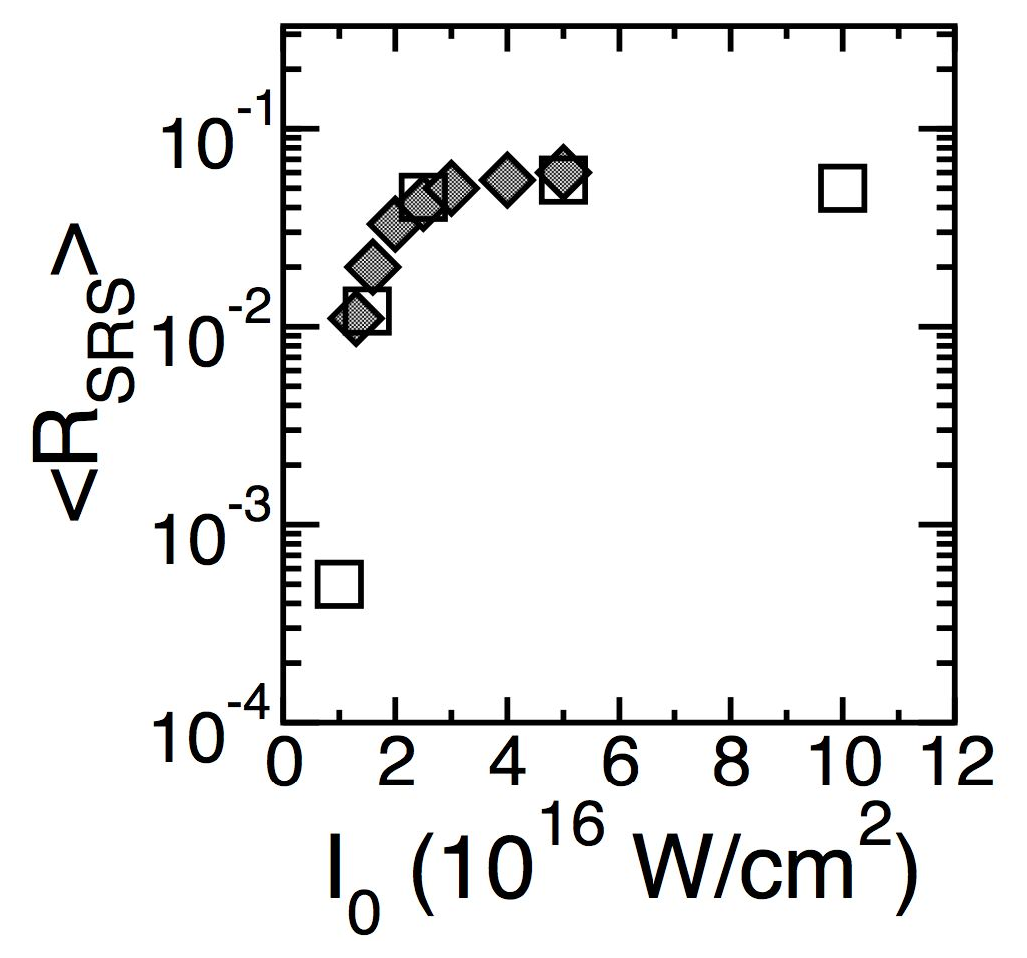
\includegraphics[height=1.375in]{figs/lpi_comparison.eps}

\vspace{0.125in}
\caption{
Bowing and self-focusing of electron plasma waves from a 3d SRS
simulation of an $f/4$ speckle.  Displayed are isosurfaces of
longitudinal electric field $E_x$ (indicating the presence of electron
plasma waves) with color indicating laser field ($E_y$).  In the
nonlinear evolution of SRS, the source for SRS backscatter
(proportional to $E_x E_y$) loses coherence, as represented by the
multi-colored isosurfaces.  Inset: SRS reflectivity as a function of
incident laser peak intensity~\cite{AAC_Conference_Paper} for laser
and plasma conditions comparable to Problems 1 and 2.  Squares
represent reflectivity obtained from runs on a homogeneous cluster of
Opteron cores (the Roadrunner ``base system,'' already deployed at
LANL); diamonds are from a \textit{suite of calculations run on
Roadrunner with higher phase-space fidelity}.  Both sets of
simulations used $136 \times 10^6$ voxels.  As expected, the observed
saturated reflectivity (the plateau) is the same, but the lower noise
afforded by higher fidelity on Roadrunner leads to reflectivity onset
at a slightly lower intensity, as predicted by
theory~\cite{Yin_et_al_Phys_Plasmas_2006}.  These science runs are a
stringent test of correctness of the Cell implementation of VPIC.
Moreover, they allow better characterization of the nonlinear onset
and saturation of SRS in NIF-like plasma conditions, the key physics
to be implemented in reduced physics models like pF3D.}
\label{fig:lpi}
\end{center}
\end{figure*}

The NIF is designed to ignite thermonuclear fuel in a laser-driven ICF
capsule, a breakthrough that will be one of the landmark achievements
in science and engineering, with a host of applications, spanning
fusion energy research, high energy density physics, and laboratory
astrophysics.  In the NIF ICF experiments, which commence in 2010,
$192$~laser beams with $1.8$~MJ of energy are directed onto the inner
walls of a hohlraum, a centimeter-sized cylindrical radiation
``bottle'' made of gold and/or uranium.  The hohlraum walls heat and
radiate x-rays, which are absorbed by a tiny ($\sim 1$~mm) capsule of
cryogenic deuterium-tritium (DT) ``fuel'' surrounded by a plastic or
beryllium ablator.  The capsule compresses to a density of hundreds of
g/cc and temperature in excess of $10$~keV, conditions under which DT
fuel can ignite.

LPI jeopardize the success of NIF fusion ignition.  As a laser beam
travels through the plasma filling the hohlraum, it scatters from and
amplifies density irregularities.  This leads to growth of parametric
instabilities that scatter laser light and degrade energy and symmetry
of capsule compression.  The most pernicious LPI are stimulated Raman
(SRS) and stimulated Brillouin (SBS) scattering, where laser light
scatters off electron and ion density fluctuations, respectively.
Indeed, the U.~S.~National Nuclear Security Administration (NNSA),
customers for this work, have reported that ``success of ICF depends
partly on mitigating the undesirable effects of two particular
parametric instabilities, stimulated Raman scattering and stimulated
Brillouin scattering.''~\cite{LLNL_LPI_webpage}

The NIF employs random phase plates to break each laser beam into a
collection of ``speckles,'' or hot spots.  To mitigate SRS backscatter
requires a predictive capability for the SRS onset threshold and
scaling of reflectivity versus laser intensity within a solitary laser
speckle.  This long-sought-after research goal is enabled for the first time
by VPIC running on the full Roadrunner platform.  This gives a unique
platform for understanding LPI that will translate into improved
predictive modeling of ICF experiments and mitigation of risk for ICF
ignition.

To put this in context, for over $30$~years, LPI has been one of the
critical issues facing ICF ignition experiments.  The current NNSA
strategy for estimating the LPI effects centers on the use of paraxial
codes, such as pF3D~\cite{Berger_Phys_Plasmas_1998}, to obtain the
amount of SRS and SBS laser backscatter in laser-driven hohlraum
plasma~\cite{Glenzer_Nature_Physics_2007,Labaune_Nature_Physics_2007}.
These codes compute SRS and SBS from analytic models with known
limitations: the models do not retain the electron trapping physics
that nonlinearly determine both the laser threshold intensity for
instability onset (above which the reflectivity increases by orders of
magnitude) or the saturation mechanism (which causes reflectivity to
saturate at high laser intensity).  In contrast, both features are
observed in \abinitio\ VPIC simulations (see the inset of
\fig{lpi}) as well as laboratory
experiments.~\cite{Montgomery_et_al_Phys_Plasmas_2002}

Only recently, with the advent of VPIC modeling of entire laser
speckles over unprecedented space and time scales, has the
state-of-the-art in kinetic plasma simulation advanced to the point
where predictive LPI modeling is possible.  This topic is of acute
interest to the ICF and high energy density physics communities and
spurred a recent Workshop on SRS and hohlraum energetics.\footnote{The
SRS Assessment Workshop, held May 7, 2008 in Livermore, California,
USA.}  One of the outcomes of the Workshop was a decision to assess
the risk to existing ICF experimental designs and initiate integration
of LPI models derived from \abinitio\ modeling of LPI into pF3D.

A predictive capability for LPI will facilitate design of ICF ignition
experiments on the multi-billion dollar NIF facility that avoid the
deleterious effects of LPI.  Moreover, it will enable rapid and
economical testing of LPI mitigation strategies, such as the use of
high-$Z$ dopant in the hohlraum fill gas, under conditions that are
difficult or expensive to assess in the laboratory.

\subsection{Plasma Physics Simulations}

In ICF experiments, LPI evolve to a complex, highly nonlinear state
involving wave-wave and wave-particle interaction; of greatest concern
are when wave-particle interactions dominate the nonlinearity.
Understanding LPI under these conditions requires high-resolution
kinetic plasma simulations that capture all of the wave-particle
physics.  These simulations must resolve complex trapped-particle
orbits and complicated structures in phase space and therefore require
the use of many particles (in some cases, as many as thousands of
particles/voxel of each species) to resolve the
dynamics~\cite{Yin_et_al_Phys_Plasmas_2006}.

Recent experiments~\cite{Kline_PRL_2005} and
modeling~\cite{Yin_et_al_PRL_2007_SRS} show that LPI in a solitary
laser speckle is represented well by a diffraction-limited laser beam.
In our 3d VPIC simulations, we launch a Gaussian diffraction-limited
laser beam from a boundary into a plasma of dimension $35 \times 6
\times 6$~$\mu$m; the simulation boundaries absorb outgoing
electromagnetic waves and reflect particles.  The $f/4$ beam
(diffraction chosen to emulate laboratory experiments and prior
calculations) is linearly polarized, of wavelength $\lambda_0 =
351$~nm, and has peak intensity ranging from $I_0 = 10^{15} -
10^{17}$~W/cm$^2$ at the center of the simulation volume.\footnote{It
is expected that the laser backscatter from daughter SRS and SBS waves
is dominated by the nonlinear dynamics of the rare speckles at very
high intensity.  While modeling of an entire laser beam within a PIC
code is impractical, we can indeed model these highest-intensity ``hot
spots.''}
% FIXME: THIS FOOTNOTE STILL NEEDS WORK.  WHAT DOES ``RARE'' SPECKLE
% MEAN?
The plasma is under-dense with electron density $n_e = 0.14
n_{\mathrm{cr}}$; here $n_{\mathrm{cr}} = c m_e / 2 \lambda_0 e^2$ is
the critical density, $c$ is the speed of light, $m_e$ is electron
mass, and $e$ is electronic charge (statcoul).  The simulation volume
spans two Rayleigh lengths in $x$, the direction of laser propagation,
and three Gaussian widths of the laser at the entrance plane in $y$
and $z$.  The electron and ion temperatures are $T_e = 4$~keV and $T_i
= 2$~keV, comparable to hohlraum plasma conditions at maximum drive
intensity.  The hohlraum is filled with plasma comprising hydrogen,
helium, and trace amounts of krypton and xenon.

The LPI simulations are at conditions $k \lde = 0.34$, where $k$ is
the wavenumber of the most unstable electron fluctuation and $\lde =
(k_B T_e / 4 \pi n_e e^2)^{1/2}$ is the Debye length ($k_B$ is
Boltzmann's constant).  The simulation time is $10^4~\wpe^{-1}$ [$\wpe
= (4 \pi n_e e^2 / m_e)^{1/2}$]; the $0.13 \times 10^6$ time steps
allow for growth of several ``bursts'' of SRS and SBS.  The simulation
volume is divided into voxels of size $1.3\lde \times 1.7\lde \times
1.7\lde$, which ensures ample resolution for the collective processes.
As appropriate for LPI simulations, the voxel mesh is uniform to avoid
laser reflection off mesh discontinuities.

We tested VPIC weak scalability and conducted a suite of science
calculations~\cite{AAC_Conference_Paper} based on the above
configuration to investigate two LPI issues: (1) What is the role
of trapped particles in the nonlinear evolution of LPI?  Can we verify
(at higher fidelity) recent
work~\cite{Yin_et_al_PRL_2007_SRS,Yin_et_al_Phys_Plasmas_2007_SRS}
showing how SRS and SBS saturate and are limited by nonlinear
wave-particle trapping that bends electrostatic wavefronts (see
\fig{lpi}), followed by transverse filamentation and break-up
of wave fronts?  (2) What is the effect on LPI of high-$Z$ dopant such
as Kr and Xe (of interest as a possible mitigation
strategy~\cite{Lushnikov_PPCF_2006} and at the hohlraum edge where Au
and U mix with low-$Z$ gas)?  In the following, ``Problem 1'' refers
to runs with $2,000$~particles/voxel per species and ``Problem 2'' is
the same problem, but at higher phase space fidelity
($6,420$~particles/voxel per species).  These numbers of
particles/voxel are comparable to published 2d studies of LPI
physics~\cite{Yin_et_al_PRL_2007_SRS,Yin_et_al_Phys_Plasmas_2007_SRS}.
In both problems, at full scale ($12,240$~cores), $31 \times
10^6$~voxels were used, with $0.31 \times 10^{12}$ and $1.0 \times
10^{12}$~particles, respectively.  The latter were three times larger
in number of particles than the next largest published PIC simulations
of plasma~\cite{Yin_et_al_PRL_2007_reconnection}.

During the initial deployment of Roadrunner at LANL, a large number of
single-laser-speckle simulations of the type described by Problems 1
and 2 (but with varying plasma conditions, laser intensity, and
diffraction) will be run and analyzed.  Therefore, it is critical to
demonstrate high performance on these problems on Roadrunner.

\section{The VPIC Particle-In-Cell Code}

VPIC uses state-of-the-art techniques of relativistic plasma
simulation~\cite{Blahovec_et_al_2000,Eastwood_et_al_1995,
Jones_et_al_1996,Kwan_Snell_1985,Nieter_Cary_2004,
Verboncoeur_et_al_1995}; these methods are briefly described below for
completeness and are discussed in more detail in
Ref.~\cite{Bowers_et_al_Phys_Plasmas_2007}.  More in-depth analysis of
PIC simulation can be found in
Refs.~\cite{Birdsall_Langdon_1985,Hockney_Eastwood_1988}.

\subsection{Model Equations}

VPIC integrates the relativistic Maxwell-Boltzmann equations in a
linear background medium:
\begin{eqnarray}
\PDeriv{f_s}{t} + 
\DotP{c\gamma^{-1}\vecu}{\Grad{f_s}} +
\DotP{\frac{q_s}{m_s c}\left(\vecE+\CrossP{c\gamma^{-1}\vecu}{\vecB}\right)}
{\Gradu{f_s}}\nonumber&\\
= \left(\PDeriv{f_s}{t}\right)_{coll}\label{eq:Boltzmann}
\hspace{2.14in}&\\
\PDeriv{\vecB}{t} = -\Curl{\vecE} \label{eq:Faraday}
\hspace{2.18in}&\\
\PDeriv{\vecE}{t} =
\eps^{-1}\Curl{\mu^{-1}\vecB} - \eps^{-1}\vecJ - \eps^{-1}\sigma\vecE.
\label{eq:Ampere}
\hspace{0.75in}&
\end{eqnarray}
Above, $f_s\left(\vecr,\vecu,t\right)$ is the phase-space density of a
species $s$ with particle charge $q_s$ and mass $m_s$.  $c$ is the
speed of light in vacuum, $\vecu$ is the normalized momentum and
$\gamma\left(\vecu\right) = \sqrt{1 + u^2}$ is the relativistic
factor.  $\vecE\left(\vecr,t\right)$, $\vecB\left(\vecr,t\right)$ and
$\vecJ\left(\vecr,t\right) = \sum_s \int d\vecu q_s c\gamma^{-1}\vecu
f_s$ are the electric field, magnetic field and current density, respectively.
$\eps\left(\vecr\right)$, $\mu\left(\vecr\right)$ and
$\sigma\left(\vecr\right)$ are the background diagonal permittivity,
permeability and conductivity tensors.
$\left(\PDeriv{f_s}{t}\right)_{coll}$ represents discrete particle
effects (e.g. short range Coulomb collisions, excitation and
ionization).

To avoid a costly direct discretization of $f_s$, PIC simulations
sample it with computational particles that typically represent many
physical particles.  \eq{Boltzmann} is replaced by the equations of
motion
\begin{eqnarray}
\Deriv{\vecr_{s,n}}{t} &=& c \gamma_{s,n}^{-1} \vecu_{s,n} \label{eq:Position}\\
\Deriv{\vecu_{s,n}}{t} &=& \frac{q_s}{m_s c} \left[
\vecE\left(\vecr_{s,n},t\right) +
\CrossP{c\gamma_{s,n}^{-1}\vecu_{s,n}}{\vecB\left(\vecr_{s,n},t\right)}
\right] \label{eq:Momentum}
.
\end{eqnarray}
$f_s$ for the computational particles obeys \eq{Boltzmann} outside of
discrete particle collisional effects.  A smooth $\vecJ$ is computed
from the particles for use in \eq{Faraday}-\eq{Ampere}.

\subsection{Model Discretization}

Time is discretized with a mixed explicit-implicit second order
splitting of \eq{Faraday}-\eq{Momentum} into operators that (in exact
arithmetic) can be individually applied exactly.  The result is a
mixture of the velocity Verlet, leapfrog, implicit Boris rotation and
exponential differencing schemes
\begin{eqnarray*}
\vecu_{s,n}\left(t^-\right) &=&\vecu_{s,n}\left(t-\delta_t/2\right) +
  \left(\delta_t/2\right)\vecE\left(\vecr_{s,n},t\right) \\
\vecu_{s,n}\left(t^+\right) &=&
  \textrm{Rotate}\,\vecu_{s,n}\left(t^-\right)\,\textrm{around}\,
  \vecB\left(\vecr_{s,n},t\right)\,\textrm{by}\\&&
  q_s\delta_t\left|\vecB\left(\vecr_{s,n},t\right)\right| /
  \left(m_s\gamma_{s,n}\right)\,\textrm{radians} \\
\vecu_{s,n}\left(t+\delta_t/2\right) &=&\vecu_{s,n}\left(t^+\right) +
  \left(\delta_t/2\right)\vecE\left(\vecr_{s,n},t\right) \\
\vecr_{s,n}\left(t+\delta_t\right) &=& \vecr_{s,n}\left(t\right) +\\&&
  c\delta_t\gamma_{s,n}\left(t+\delta_t/2\right)^{-1}
           \vecu_{s,n}\left(t+\delta_t/2\right) \\
\vecB\left(t+\delta_t/2\right) &=&
  \vecB\left(t\right) -
  \left(\delta_t/2\right)\Curl{\vecE\left(t\right)} \\
\vecE\left(t+\delta_t\right) &=&
  e^{-\delta_t\eps^{-1}\sigma}\vecE\left(t\right) + 
  \eps^{-1}\left(1-e^{-\delta_t\eps^{-1}\sigma}\right) \\
&&\left( \Curl{\mu^{-1}\vecB\left(t+\delta_t/2\right)} -
         \vecJ\left(t+\delta_t/2\right) \right) \\
\vecB\left(t+\delta_t\right) &=& \vecB\left(t+\delta_t/2\right) -
  \left(\delta_t/2\right)\Curl{\vecE\left(t+\delta_t\right)}
.
\end{eqnarray*}

The simulation domain is divided into a regular mesh of identical
rectangular voxels with potentially irregular but voxel aligned
boundaries.  Because $\vecJ$ is smooth, $\vecE$, $\vecB$ and $\vecJ$
can be sampled on this mesh and interpolated between the mesh and
particles.  Particle fields are interpolated with an ``energy
conserving'' scheme; for example, $E_x$ is bilinearly interpolated
from the four Yee-mesh $E_x$ edge samples and $B_x$ is linearly
interpolated from the two Yee-mesh $B_x$ face samples of the voxel
containing a particle.  This scheme is especially efficient in
simulations with irregular boundary conditions as it uses no field
samples outside the voxel containing a particle.  Yee-mesh $\vecJ$
samples are extrapolated from the particles by the method of
Villasenor and Buneman~\cite{Villasenor_Buneman_1992}; a particle
makes a $\vecJ$ contribution in each voxel through which it passes.
Though expensive, this reduces artifacts from the accumulation of
Gauss' law ($\Div{\eps\vecE}=\rho$) violations and provides efficient
and robust particle boundary interaction detection.  A variety of
particle and field boundary conditions are supported including
particle absorbing, particle reflecting, particle refluxing, perfect
electric conductor, perfect magnetic conductor, field emitting and
field absorbing (first order Higdon~\cite{Higdon_1986}).

The rotation above can be done efficiently with a modified Boris
push~\cite{Boris_1970}.  To avoid aliasing of cyclotron motion above the
simulation Nyquist frequency to lower frequencies, VPIC uses an
efficient energy conserving sixth order rotation angle approximation
like that in Ref.~\cite{Blahovec_et_al_2000}.

The curls are computed with second order finite differencing.  This
and the method of Villasenor and Buneman imply a discretized Gauss'
law.  However, finite precision arithmetic error can cause small
Gauss' law violations to accumulate.  VPIC periodically applies Marder
passes~\cite{Marder_1987} tuned specifically to clean these
violations.  While this method is local and inexpensive, it suffices
to use it infrequently to keep this law satisfied to near machine
precision.  For wavelengths comparable to the voxel dimensions, the
discretized speed of light can deviate significantly from $c$;
allowing relativistic particle motion to generate non-physical
Cherenkov radiation at these wavelengths.  VPIC uses the transverse
current adjustment method~\cite{Eastwood_et_al_1995} to damp
non-physical Cherenkov radiation while leaving the discretized charge
conservation properties unchanged.

In vacuum, the field advance reduces to a basic FDTD
algorithm~\cite{Yee_1966} and the time step and voxel dimensions must
satisfy the Courant condition, $\left(c\delta_t/\delta_x\right)^2 +
\left(c\delta_t/\delta_y\right)^2 + \left(c\delta_t/\delta_z\right)^2
< 1$.  Additionally, the particle advance usually requires the time
step and voxel dimensions to satisfy $\omega_p \delta_t < 2$ and
$\delta_{x,y,z} \approx \lambda_d$ where $\omega_p$ is the peak plasma
frequency and $\lambda_d$ is the plasma Debye
length~\cite{Birdsall_Langdon_1985,Hockney_Eastwood_1988}.  Given that
particles cannot exceed $c$, satisfying both the Courant and Debye
conditions is typically sufficient.  Though the time step is stable
for any cyclotron frequency, it is usually resolved for accurate
dynamics.  Sampling $f_s$ can require over thousands of particles per
voxel, depending on the above and the phenomena being studied, to avoid
enhanced computational particle collision rates and to fully resolve
resonant kinetic phenomena.

\subsection{Comparison with other simulation techniques}

Monte Carlo, fluid dynamics and molecular dynamics (MD) techniques can
also be used to simulate plasma systems or, more generally, systems
modeled by the Boltzmann equation.  Though amenable to embarrassingly
parallel computation, Monte Carlo techniques are best at computing
equilibrium properties and thus not suited for examining the
non-equilibrium time-dependent dynamics of LPI.  Though less expensive
than PIC, the equations of state (which relate quantities like
pressure to density and temperature) used in fluid dynamics neglect
the detailed phase-space dynamics critical to wave-particle LPI
processes.

The simulation technique most related to PIC is MD.  The primary
difference is that short range particle-particle interactions are
explicitly computed and long range particle-particle interactions are
often approximated in MD (e.g. atoms interacting via a Lennard-Jones
potential), while the converse is true in PIC (e.g. high temperature
plasma where long range collective interactions among charged
particles dominate over short range interactions).  Computationally,
the impact is, even compared to MD techniques whose operations per
time step scale as $O(N)$ (where $N$ is the number of particles), that the
amount of computation necessary per particle per time step is much
lower than MD.  While being a net benefit for systems amenable to PIC
simulation, this makes it harder to achieve high raw performance due
to data motion limitations on modern supercomputers.

\section{VPIC Implementation}

\begin{table}
\caption{VPIC implementation rules of thumb.}
\begin{center}
\begin{tabular}{l r r r r r r}
\hline
\hline
\multicolumn{3}{c}{Operation}  & & Time        & & Rel.~Cost \\
\hline
Data access      & & Internode & & 10,000   ns & &   100,000 \\
(Latency)        & &    Memory & &     50   ns & &       500 \\
                 & &  L2 Cache & &      5.0 ns & &        50 \\
\vspace{4pt}     & &  L1 Cache & &      1.0 ns & &        10 \\
Data movement    & & Internode & &      5.0 ns & &        50 \\
(32-bit)         & &    Memory & &      0.5 ns & &         5 \\
                 & &  L2 Cache & &      0.2 ns & &         2 \\
\vspace{4pt}     & &  L1 Cache & &      0.1 ns & &         1 \\
Single precision & &      FLOP & &      0.1 ns & &         1 \\
\hline
\end{tabular}
\end{center}

Data access estimates the time to initiate a transfer between the
processor and a level in its memory hierarchy.  Data movement
estimates the time to move the next $32$~bits in a transfer.
Internode figures were obtained from benchmarks of typical high
performance cluster interconnects.  The single precision FLOP figure
corresponds to a $2.5$~GHz processor completing a 4-vector SIMD
instruction every clock.  Other rules of thumb were similarly
extrapolated from various data sheets and benchmarks.
\label{tbl:rules-of-thumb}
\end{table}

Most modern supercomputers consist of a large number of nodes
connected by a network.  The nodes themselves contain one or more CPUs
and memory.  CPU performance has improved more rapidly than memory
performance over recent decades.  To compensate, modern CPUs use a
deep memory hierarchy with faster (though smaller and more limited)
``cache'' memories located close to the CPU.  As shown in
\tbl{rules-of-thumb}, optimizing data access is critical; achieving
high performance requires minimizing the number of internode
communications, number of memory accesses, amount of data in internode
communications, amount of memory accessed and number of arithmetic
operations, in roughly that order.

In contrast to embarrassingly parallel simulations, due to the
emphasis on long range interactions, communication between nodes is
necessary at every time step in PIC simulations.  Fortunately, due to the
finite $c$ in relativistic simulations, internode communications are
naturally optimized by a spatial domain decomposition.  Nodes need
only communicate with neighboring nodes and no global communications
or barriers are required.  As a result, optimizing memory access is
the greatest technical challenge in high performance PIC simulation, as
there is typically more field and particle data per node than can fit
in any cache on that node.  Minimizing local data motion requires
grouping data needed to perform operations contiguously and accessing
it sequentially when possible.  As computation and storage are cheap
compared with data motion, replicating computations and/or data is
often worthwhile.

\subsection{Data motion optimization}

Single precision codes can often be made to run faster than their
double precision equivalents, as single precision requires half the
data movement, and most modern CPUs provide single precision 4-vector
SIMD capabilities.  For typical time steps, voxel dimensions and
particles per voxel, model discretization error exceeds single
precision arithmetic error.  Thus, single precision should usually be
acceptable provided it does not introduce non-physical artifacts
(e.g. large violations of otherwise conserved quantities).

VPIC uses single precision to help achieve high performance but takes
care to structure calculations to maximize accuracy.  One example is
that particle coordinates are stored as a voxel index plus a
normalized offset from the center of that voxel; this gives over three
orders of magnitude improvement in the worst case absolute position
resolution seen by a particle for simulations of interest compared to
a more common global coordinate system position
representation.\footnote{In exact arithmetic, the index+offset
representation is equivalent to the more common global coordinate
system representation.  As such, there are no abrupt changes in
Jacobians as particles move from voxel to voxel.  Interestingly, each
voxel has identical numerical properties regardless how the voxel mesh
is translated, oriented or reflected in absolute
coordinates---avoiding symmetry breaking spatially dependent
arithmetic errors that can corrupt single precision simulations using
global coordinate system position representations.}  Beyond reducing
numerical errors, this representation accelerates operations like
field interpolation (though it does require that the coordinate system
for a particle's offset be updated whenever that particle crosses into
a different voxel).

Another example is that particle velocity is stored as the
relativistic particle momentum normalized by $mc$.  Unlike a quantity
linearly proportional to velocity, the normalized momentum is not
bounded.  This avoids issues with both discretization and arithmetic
error, especially for particles moving very close to $c$.  In
practice, single precision has not been an issue for production use of
VPIC and even more precision demanding computations have successfully
used single precision as
well~\cite{Bowers_et_al_2006,Langou_et_al_2006,Lippert_et_al_2007}.
Based on extensive verification and validation studies of VPIC LPI
simulations~\cite{Yin_et_al_Phys_Plasmas_2006}, we have high
confidence that single precision is more than adequate for the
problems described previously.

Since there is more particle data than can fit in any cache, it is
desirable to limit the number of times a particle is touched during a
time step lest performance be limited by moving particle data to and
from memory.  This can be achieved by processing the majority of the
particles in a single pass.  Give the above discretization, the inner
loop of VPIC conceptually is:
\begin{verbatim}
for all particles,
  interpolate the particle fields
  update the particle momentum
  compute the particle motion
  if the particle motion is exceptional,
    update the exception list
  else
    update the particle position
    update the current
  end if
end for
\end{verbatim}
To further minimize particle data moving costs, particles are stored
contiguously, memory aligned and organized for 4-vector SIMD.  Given
this and the above, particles for a given species are stored in an
aligned 1d array of structures of the form:
\begin{verbatim}
struct {
  float dx, dy, dz; int32_t i;
  float ux, uy, uz, q;
};
\end{verbatim}
As a result, the inner loop streams through particle data once using
large aligned memory transfers under the hood---the ideal memory
access pattern.

\begin{figure*}
\begin{center}
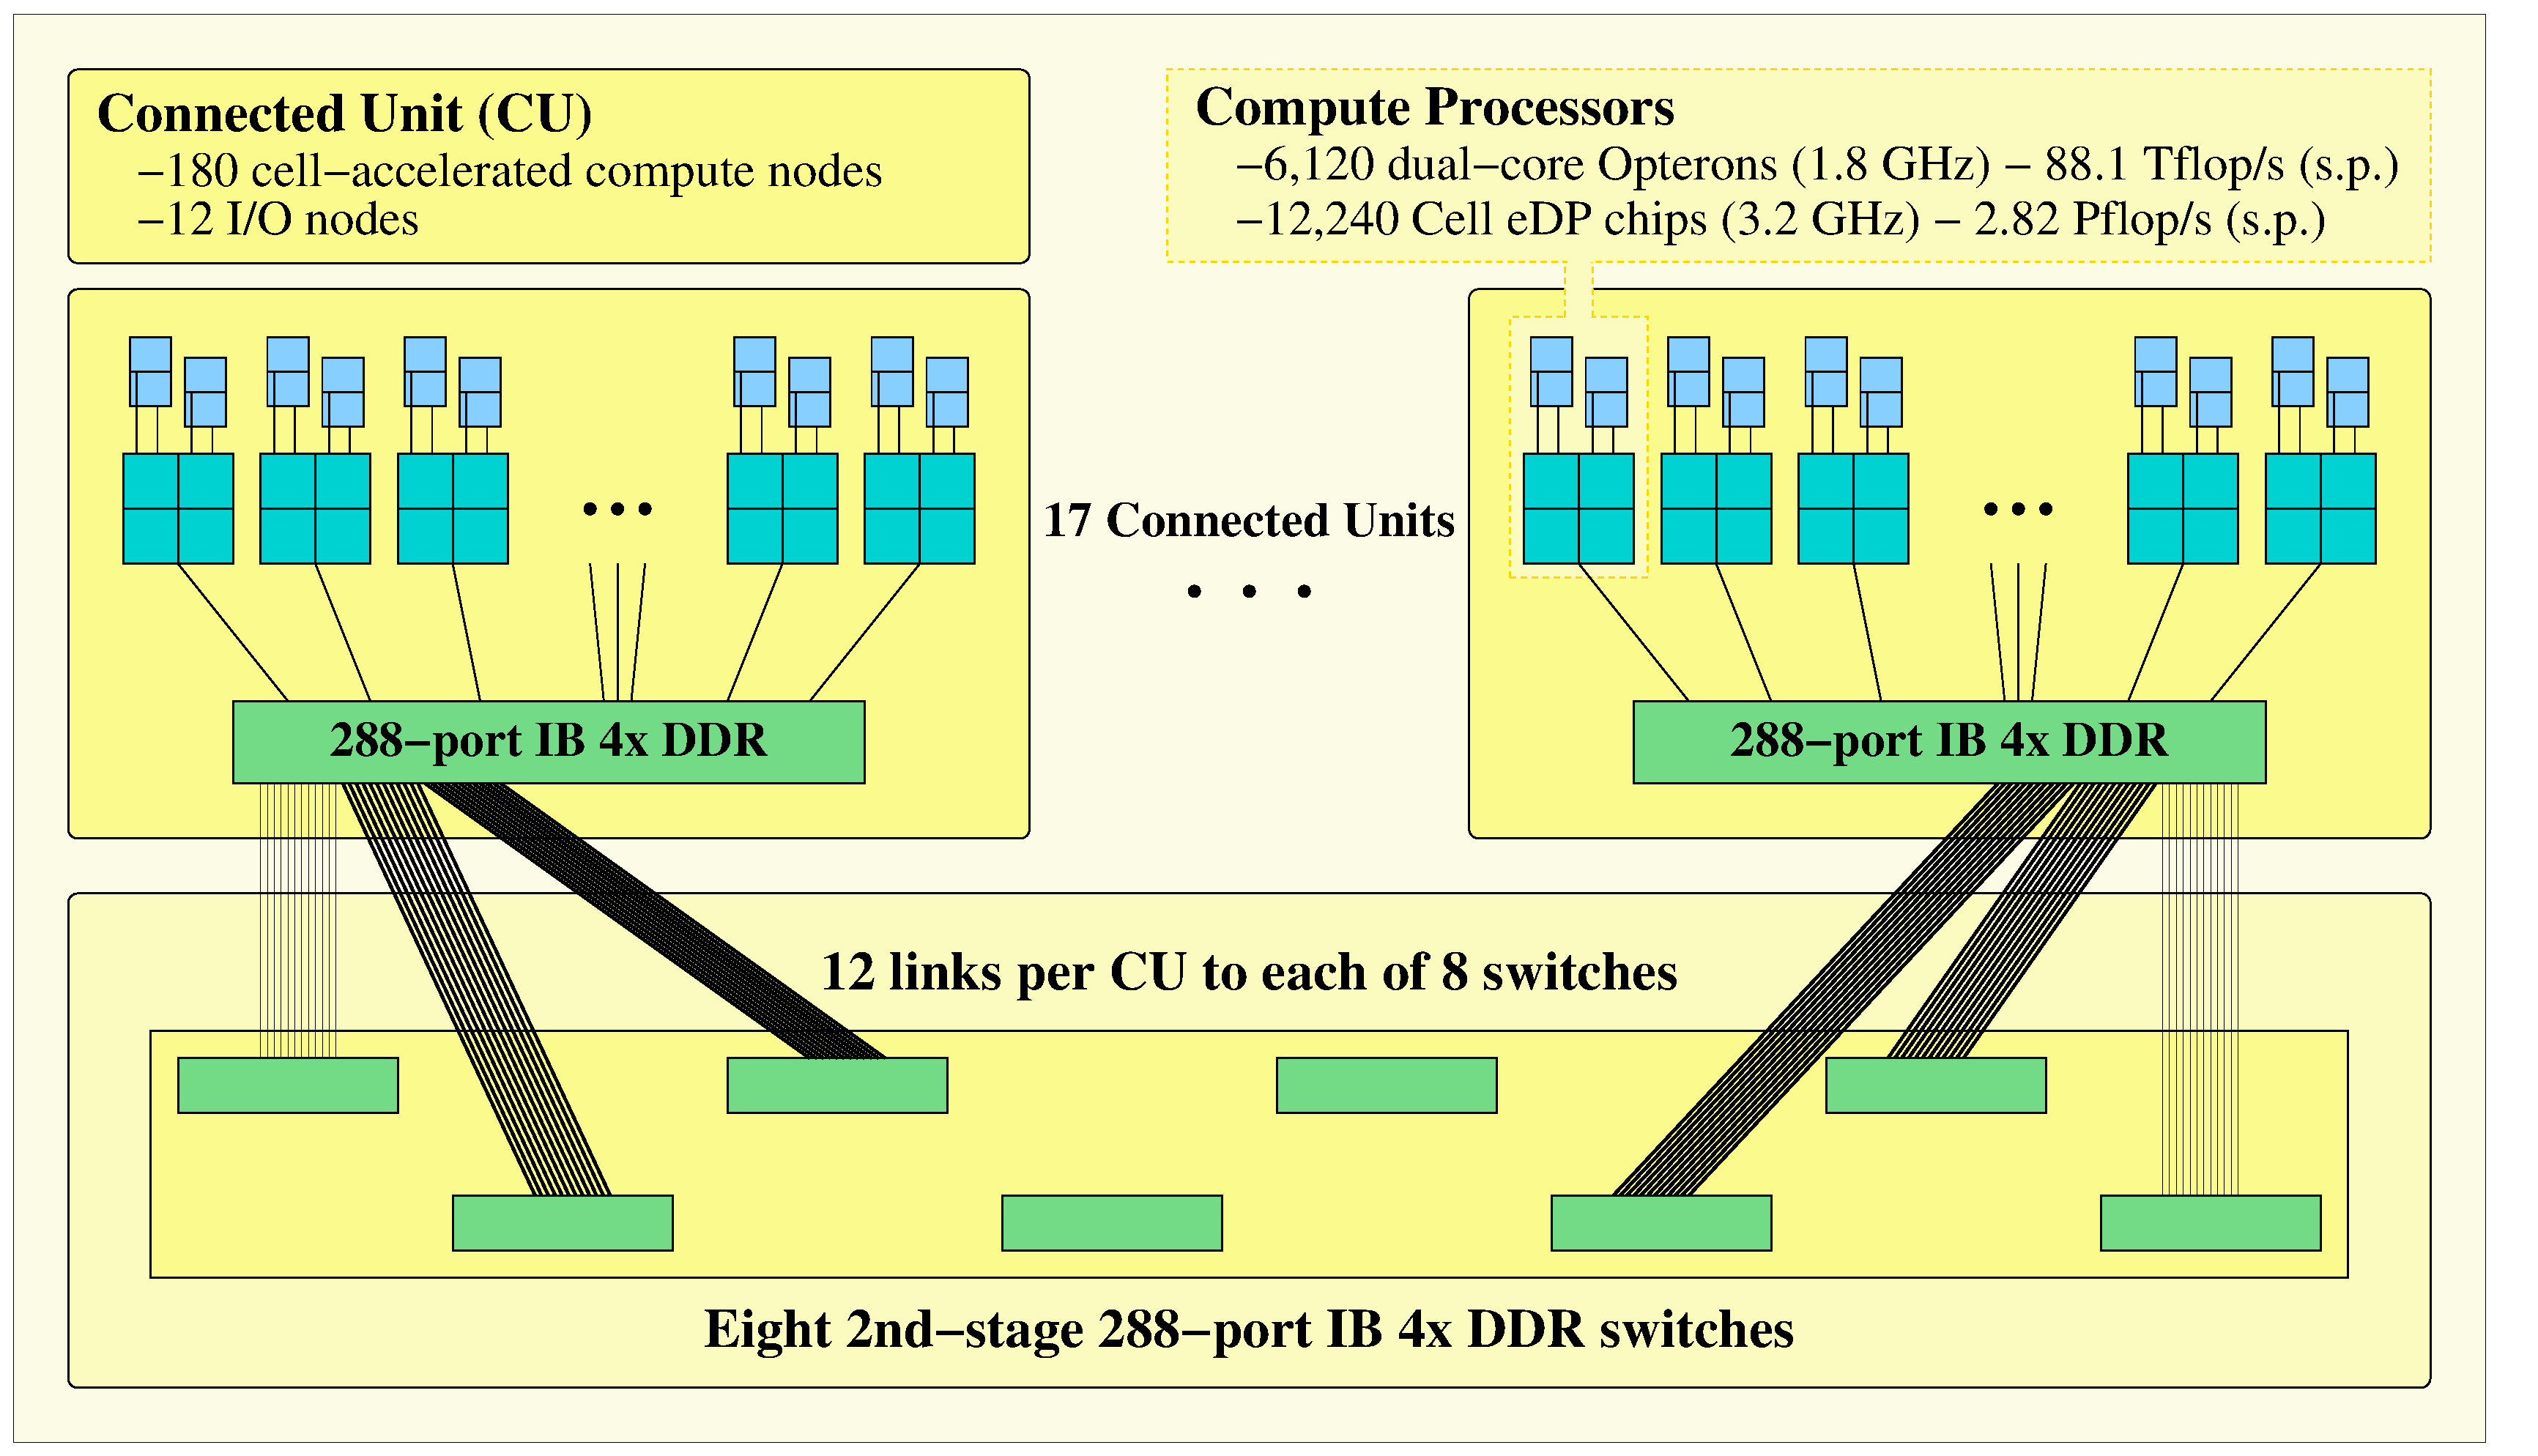
\includegraphics[width=7in]{figs/system.eps}
\caption{Roadrunner System Overview --- Roadrunner is a collection
of $17$~Connected Units of $180$~Triblade compute nodes connected by
an Infiniband backplane.  Each Triblade has $4$~Opteron cores and
$4$~Cell eDP chips. Thanks to Kenneth R. Koch for original figure.}
\label{fig:system}
\end{center}
\end{figure*}

Field interpolation can likewise severely impact performance.  If
particles are stored in a random order, field samples will be accessed
in a random order.  Because field samples do not fit within cache,
these accesses will often require memory transfers.  The situation is
made worse if field samples are directly accessed, as several
non-contiguous memory transfers may be necessary.  Worse still is if
the field components are stored in separate arrays; in this worst
case, VPIC's field interpolation could involve up to $13$~memory
transfers per particle.  Further exacerbating this, more data than
requested would be transferred as modern CPUs tend to round-up small
memory transfers to the cache line granularity.  To make field
interpolation efficient, in addition to the index+offset particle
position representation, an array of interpolation coefficients is
precomputed and saved in a contiguous, aligned, 4-vector SIMD
compatible layout:
\begin{verbatim}
struct {
  float ex, dex_dy, dex_dz, d2ex_dydz;
  float ey, dey_dz, dey_dx, d2ey_dzdx;
  float ez, dez_dx, dez_dy, d2ez_dxdy;
  float cbx, dcbx_dx, cby, dcby_dy;
  float cbz, dcbz_dz, pad0, pad1;
};
\end{verbatim}

Additionally, the particle array is periodically sorted by the
containing voxel index.  Because the particles do not move far per
time step, sorting is infrequent---every tens to hundreds of time
steps.  Nevertheless, the sorting can be done efficiently both
in-place and out-of-place in $O(N)$ operations~\cite{Bowers_2001}.  As
a result, all the particles in a given voxel are processed
approximately consecutively; the interpolation coefficients necessary
for these particles will be loaded once from memory and cached.
Additionally, the interpolation coefficients themselves are accessed
approximately sequentially in large aligned transfers a near minimal
number of times.  Even though precomputing the interpolation
coefficients requires over three times the storage as the raw field
samples, the net impact is to reduce memory transfers to minimal
levels by making more efficient use of cache.

\subsection{SIMD optimization and exceptions}

Given single precision and SIMD compatible data layouts, all particle
processing described above is ideal for 4-vector SIMD.  However,
languages like C and FORTRAN are not expressive enough (e.g. data
alignment restrictions) to allow compilers to use 4-vector SIMD in
operations as complex as those in VPIC.  To compensate, VPIC has a C
language extension that allows portable 4-vector SIMD code to be
written and converted automatically to high performance 4-vector SIMD
instructions on a wide variety of platforms.  A similar approach was
used in Ref.~\cite{Bowers_et_al_2006}.

Unfortunately, $\vecJ$ accumulation is not as SIMD friendly.
Determining the voxels through which a particle has passed varies: one
particle might remain in the voxel in which it started, while the next
might cross through several in a time step.  Fortunately, particles
cross voxel boundaries infrequently.  VPIC uses 4-vector SIMD to
advance and accumulate $4$~particles at a time, making the assumption that
none of the
$4$~particles cross any boundaries.  Particles that do are detected
and make no $\vecJ$ contribution during this process.  During
subsequent $\vecJ$ accumulation of voxel crossing particles, if a
particle hits an ``exceptional'' boundary (e.g. needs to be sent to
another node), the particle index and remaining displacement are saved
for later processing.  No additional passes through the particles are
necessary to find exceptions.  Thus, exception handling (often slow
and application specific) is cleanly separated and does not pollute
the instruction or data caches during the particle advance.  Like the
interpolation coefficients, $\vecJ$ contributions from particle motion
in a voxel are made to a contiguous, aligned set of partial currents,
which is then post-processed into $\vecJ$ prior to the field advance;
the same benefits described for interpolation coefficients apply.

\section{Roadrunner overview}

The Roadrunner supercomputer, shown in \fig{system}, is a hybrid,
petascale system to be deployed at Los Alamos National Laboratory in
2008.  The system is a first-of-its-kind, heterogeneous
cluster-of-clusters that utilizes a combination of $6,120$, $1.8$~GHz,
dual-core AMD Opteron \emph{host} CPUs with $12,240$, $3.2$~GHz, IBM
\emph{PowerXCell 8i accelerator} CPUs also known as the Cell
\emph{extended Double Precision (eDP)} CPU.  Roadrunner has a
theoretical peak performance of $2.82$~Pflop/s in single
precision.\footnote{This does not include the Opteron host CPUs, which
have an additional theoretical peak performance of $0.0881$~Pflop/s in
single precision.}  The Roadrunner supercomputer is the first machine
to achieve a sustained petaflop on the TOP500 LINPACK benchmark used
to rank the fastest supercomputers in the world~\cite{top500}.

\subsection{Cell Broadband Engine Architecture (CBEA)}

% DO NOT INCLUDE UNLESS WE HAVE SPECIFIC PERMISSION BY IBM
%\begin{figure*}
%    \begin{center}
%    \scalebox{0.5}{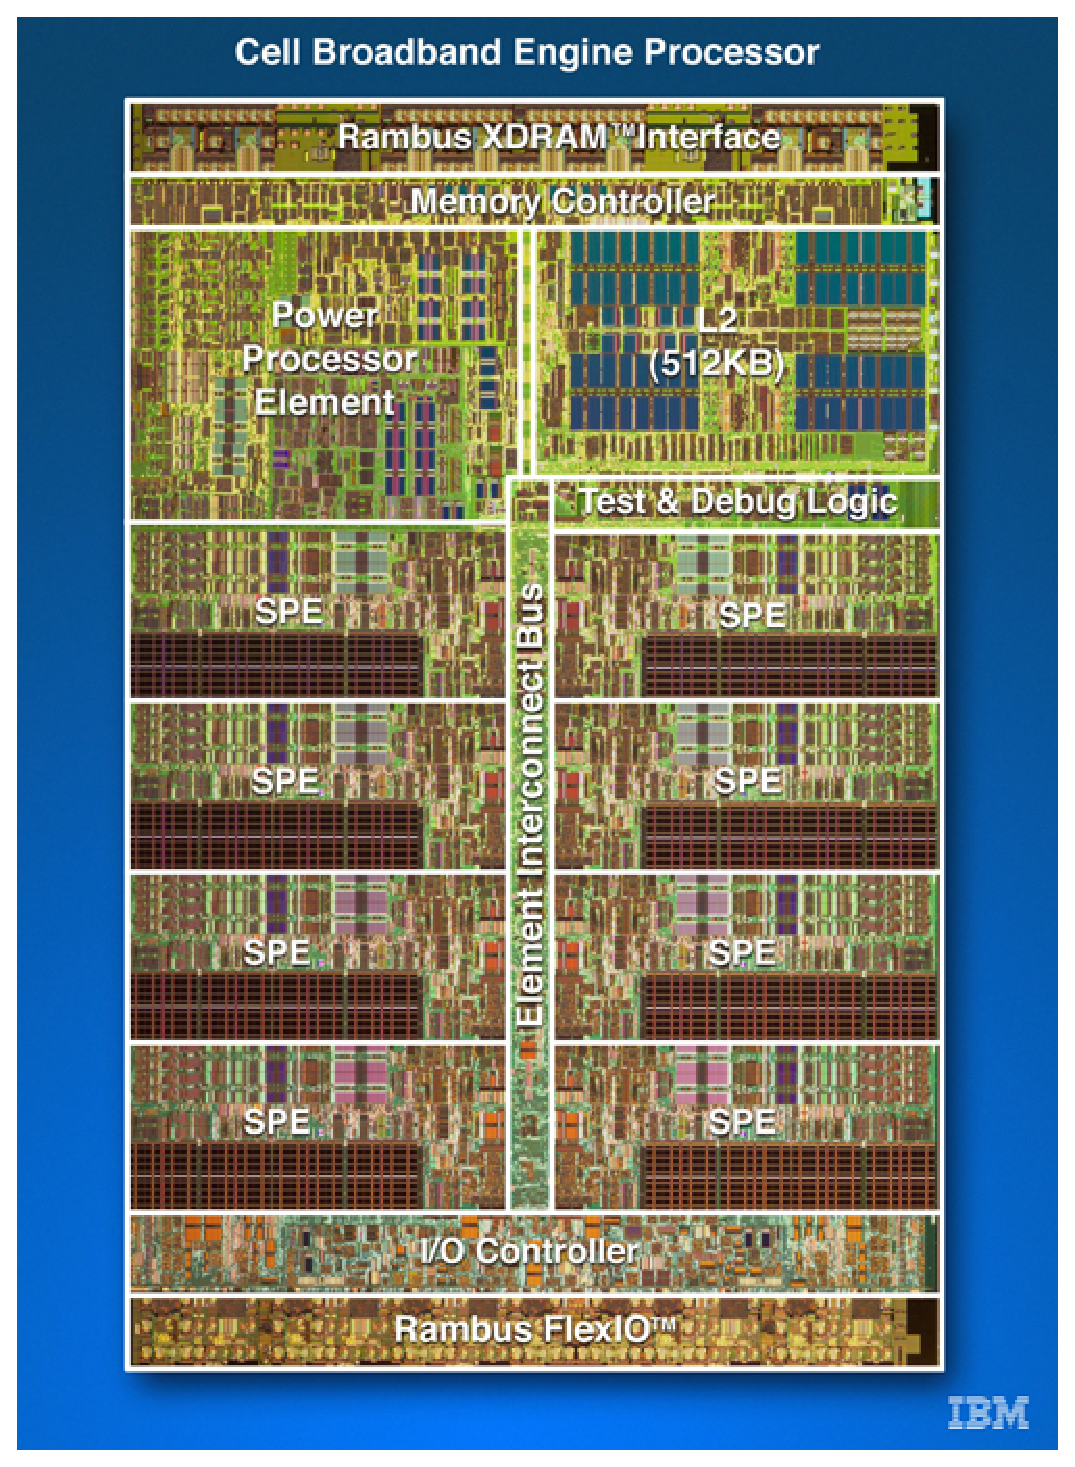
\includegraphics{cell}}
%    \caption{Cell Broadband Engine}
%    \label{fig:cell}
%    \end{center}
%\end{figure*}

The \emph{Cell Broadband Engine (Cell BE)}, developed jointly by Sony
Computer Entertainment, Toshiba, and IBM, is an ($8+1$)-way
heterogeneous parallel CPU that incorporates eight
\emph{synergistic processing elements (SPEs)} and one
\emph{power processing element (PPE)} connected via an
\emph{Element Interconnect Bus (EIB)}.  The EIB also connects
a memory controller (MIC) and two off-chip I/O interfaces.  This CPU
is used in the Sony Playstation 3 gaming console, and is currently
offered in products from IBM (QS21 blade) and Mercury Computer Systems
(CAB PCI-e card and DCBB2 blade)~\cite{mercury}.  IBM has developed an
enhanced double precision version of the Cell BE chip specifically for
use in supercomputers like Roadrunner, the PowerXCell 8i (Cell eDP).
Except as regards double precision performance, the Cell eDP does not
differ significantly architecturally from the Cell BE.

The PPE is a modestly provisioned general purpose core which serves as
a controller for the eight SPEs.  It supports two execution threads and
has a theoretical peak performance of $25.6$~Gflop/s single precision
($6.4$~Gflop/s double precision) at $3.2$~GHz.  Each SPE core has dual
$128$~bit vector execution pipelines, a $128$~entry register file and
$256$~KB user-controlled, embedded SRAM called the \emph{Local Store
(LS)}.  Each SPE has a theoretical peak performance of $25.6$~Gflop/s
single precision ($12.8$~GFlop/s double precision) at $3.2$~GHz.  All
data and text operated on by a SPE must be fetched from main memory to
the SPE's LS using \emph{direct memory access (DMA)} calls.  Each SPE
has its own $32$~channel \emph{Memory Flow Controller (MFC)} that
supports up to $12$~outstanding DMA requests and has a theoretical
bandwidth of $25.6$~GB/s to DRAM.

\subsection{Triblades}

Roadrunner's CPUs are hosted on $3,060$~\emph{Triblade} compute nodes.
A Triblade, shown in \fig{triblade}, actually integrates four physical
blades: one IBM LS21, dual-socket Opteron blade, one expansion blade,
and two IBM QS22 Cell blades.  The expansion blade connects the two
QS22s to the LS21 via four PCI-e x8 links and provides the node's
ConnectX IB 4x DDR link.  Each PCI-e x8 link logically connects an
Opteron core to a Cell eDP CPU---there is a one-to-one relationship
between Opteron cores and Cell eDP CPUs---with a theoretical bandwidth
of $2$~GB/s.  The LS21 blade incorporates two dual-core AMD Opteron
CPUs running at $1.8$~GHz with $4$~GB DDR2-667 DRAM per core.  Each
QS22 blade has two Cell eDP CPUs running at $3.2$~GHz with $4$~GB
DDR2-800 DRAM per Cell CPU.

\begin{figure}
\begin{center}
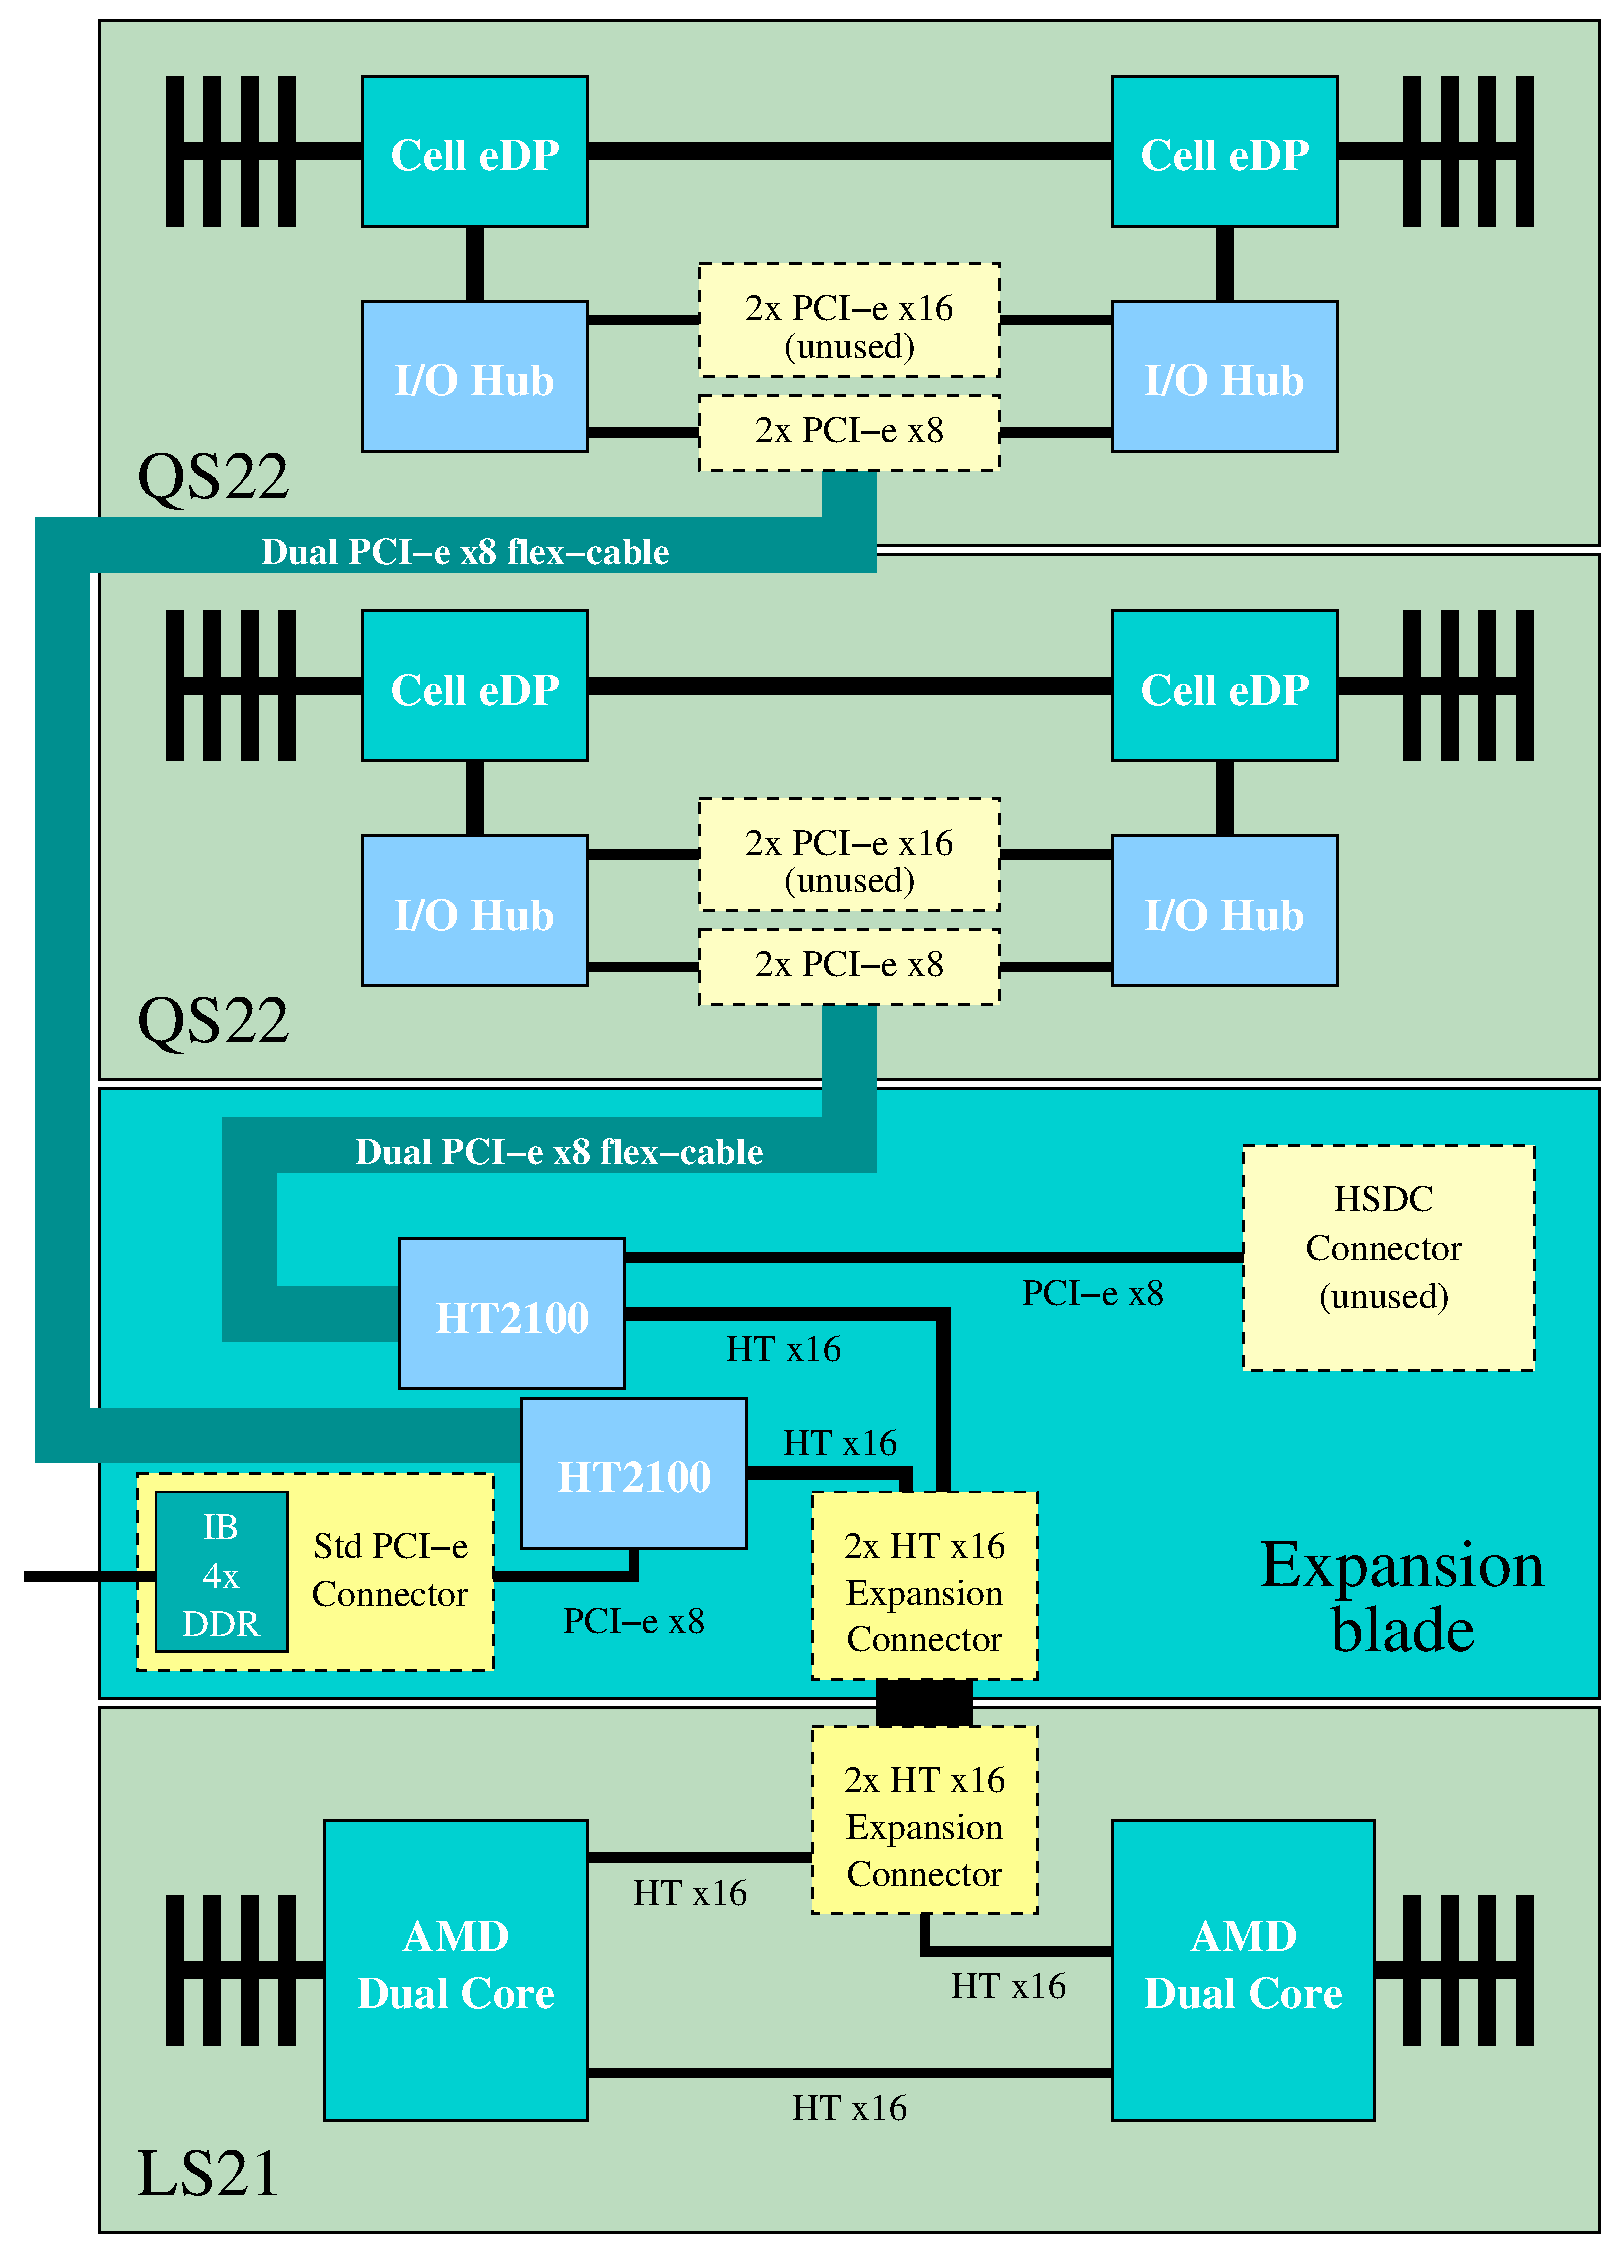
\includegraphics[width=3.375in]{figs/triblade.eps}
\caption{Triblade Compute Node.  Each Cell eDP CPU is logically
connected to an Opteron core with a theoretical bandwidth of
$2$~GB/s.  Thanks to Kenneth R. Koch for original figure.}
\label{fig:triblade}
\end{center}
\end{figure}

\subsection{Connected Units}

Roadrunner's Triblades are organized into $17$~\emph{Connected Units
(CU)}.  A CU consists of $180$~Triblades and $12$~I/O nodes linked by
a $288$~port Voltaire Infiniband 4x DDR switch.  A CU is a powerful
cluster in its own right, with a single precision theoretical peak
performance of $165.9$~Tflop/s (double precision peak of
$82.9$~Tflop/s); a single CU would rank in the top $30$ of the June
2008 TOP500 list.

The CUs are connected via eight second-stage $288$~port Voltaire
Infiniband 4x DDR switches.  This allows for $12$~links per CU to each
of the eight switches, with $192$~ports \emph{in} and $96$~ports
\emph{up}, creating a two-to-one over-subscribed, fat-tree network
topology.

\section{Porting to Roadrunner}

\begin{figure}
\begin{center}
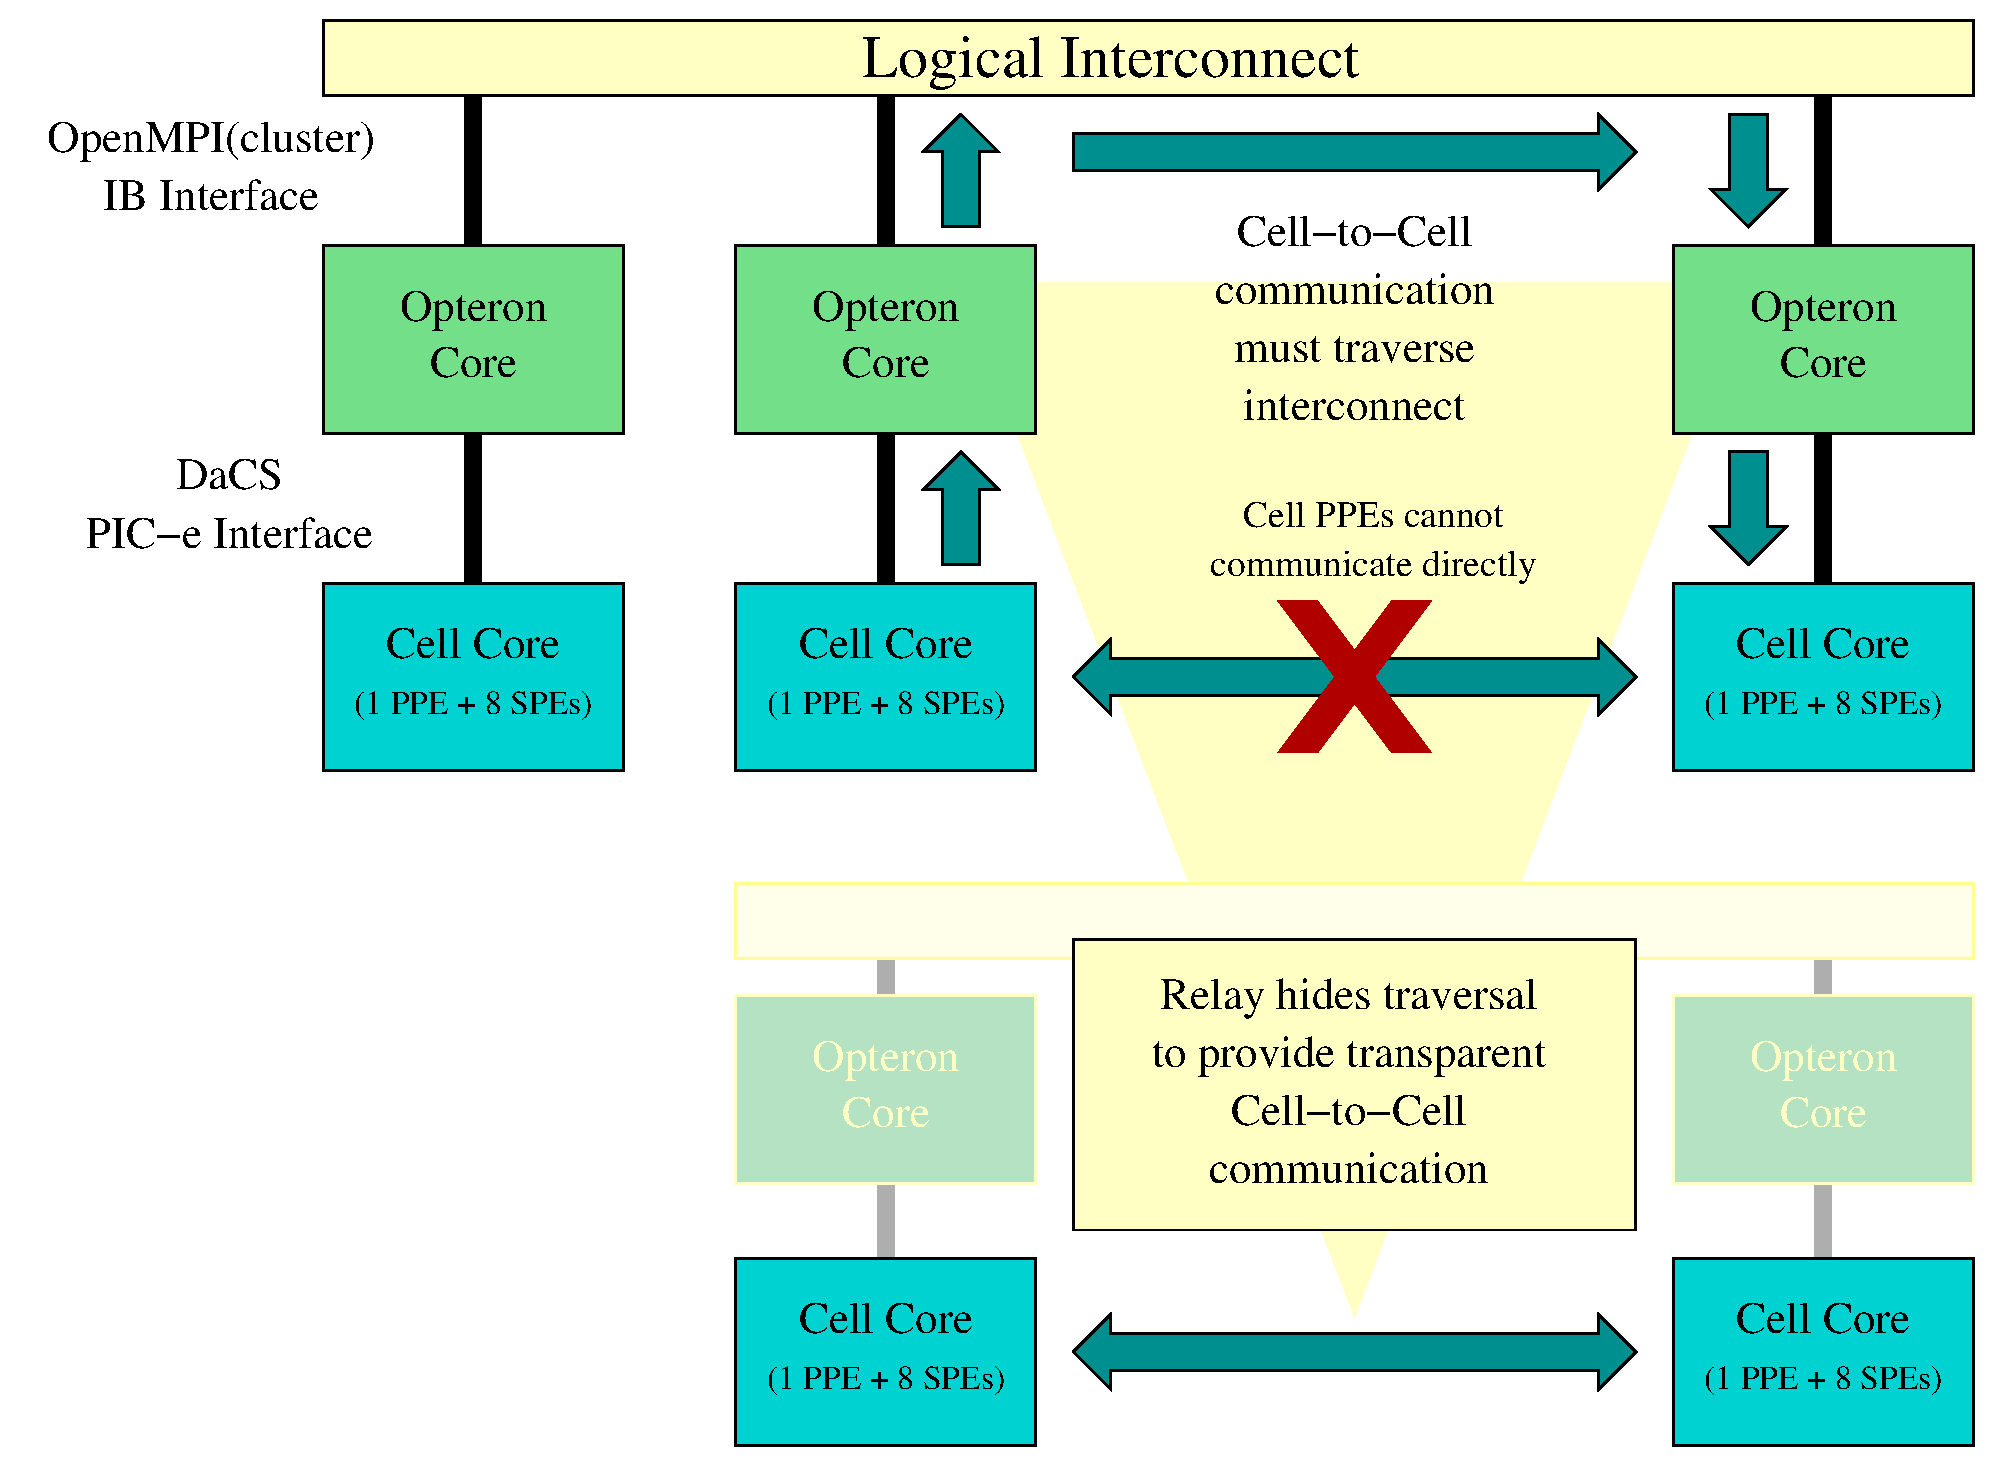
\includegraphics[width=3.5in]{figs/relay.eps}
\caption{MP Relay allows VPIC to be utilized on heterogeneous
machines like Roadrunner as well as conventional homogeneous
clusters.}
\label{fig:relay}
\end{center}
\end{figure}

\subsection{General strategy}

In VPIC, performance is asymptotically limited by the rate particles
can be streamed to and from DRAM.  On Roadrunner, the bandwidth
between the Cell CPU and Cell local DRAM greatly exceeds the bandwidth
between the Cell CPU and Opteron local DRAM (limited by the
PCI-Express bridge).  However, the Cell CPU to Cell CPU bandwidth is
limited by the internode Infiniband connection.  Accordingly, in
porting VPIC to Roadrunner, we decided (1) all local simulation state
would reside within Cell DRAM, (2) the Cell CPUs would be responsible
for all simulation computations and (3) the Opterons would manage
communications among Cell CPUs.  This maximizes the bandwidth between
Cell CPUs and simulation state.  It also is less complicated to
implement and allows VPIC to be used on Cell-only clusters.

To execute this strategy, we developed a message relay layer called
\emph{MP Relay} that runs on the Opterons and handles forwarding of
message traffic and remote I/O for the QS22 blades.  As shown in
\fig{relay}, MP Relay flattens the hierarchical network topology of
Roadrunner, making it possible to use the same underlying VPIC
implementation on Roadrunner, clusters of Cell CPUs, and traditional
clusters with very little architecture specific code.  The PPE handles
communication for the Cell CPU through an abstracted message passing
layer.  Communication between Opterons and Cells is handled within the
message passing layer using the IBM \emph{Data, Communication, and
Synchronization (DaCS)} library.  Communication among Opterons uses
MPI.  Under \emph{MP Replay}, the zero-byte latency from Cell PPU to
Cell PPU (across Triblades) was measured to be $10.6$~$\mu$s and a
bandwidth of $1$~GB/s was measured for $1$~MB message sizes on
pre-production hardware.

\subsection{Particle advance kernel}

Since the particle advance is the dominant cost in VPIC, it was the
focus of initial porting efforts.  To process a particle list, the SPEs
are assigned approximately equally sized non overlapping segments of
the list and their own set of partial currents to accumulate.  Each
segment contains a multiple of $16$~particles; the PPE advances any
left overs while the SPEs are working.  Particle data are triple
buffered on the SPEs in blocks of up to $512$~particles (at most
$16$~KB are needed to hold a block---the largest size of a single DMA
transfer).  While a block is processed, the next is loaded and the
previous is stored.  Block processing groups particles by $4$ and uses
4-vector SIMD to advance them (as done on conventional CPUs).  To
minimize stalls and utilize fully an SPE's register file and dual
execution pipelines, the vectorized inner loop is hand unrolled and
modulo scheduled by $4$.  As a block is guaranteed to contain a
multiple of $16$~particles, no code is needed to process left over
particles on the SPEs.

The challenge of SPE particle processing is handling random memory
access and particle exceptions.  Each SPE's ``local store'' is
analogous to cache, but, unlike conventional cache, memory transfers
must be explicitly managed through the MFC.  Though non-trivial, this
makes it possible to design high performance application specific
cache protocols~\cite{Kahle_et_al_2005}.  A $512$~line software cache
of read-only interpolation coefficients, read-only voxel adjacencies
and read-write partially accumulated currents handles random memory
access.  The cache has a fully associative least recently used (LRU)
policy; a line can hold any voxel's data and the least recently used
line is replaced when caching new data.  The cache has a simple
software interface: \verb+voxel_cache_fetch+ and
\verb+voxel_cache_wait+.

\verb+voxel_cache_fetch+ initiates DMA transfers to evict the LRU
cache line and replace it with the requested voxel's data.  It returns
the cache line where the data will be stored.  \verb+voxel_cache_wait+
waits until all pending cache DMA transfers are complete.  Because the
cache is fully associative and LRU, it is easy to determine what is
cached; the last $512$~unique requests are guaranteed to be cached
after a call to \verb+voxel_cache_wait+ and before any new calls to
\verb+voxel_cache_fetch+.  Accordingly, before block processing,
\verb+voxel_cache_fetch+ is called for each voxel referenced in the
block followed by a \verb+voxel_cache_wait+.  Because the particle
list is approximately sorted, most of these will be cache hits.
Regardless, the cache is large enough that, even if every particle in
a block was in a different voxel, all voxel data is guaranteed to be
in cache once block processing begins.

Under the hood, \verb+voxel_cache_fetch+ queries a hash table to
determine if the requested voxel is already cached.  This hash table
is oversized to reduce collisions and uses linear probing and modular
hashing for implementation efficiency.  If a cache hit occurs, the cache line
replacement order (stored as a doubly linked circular queue) is
updated.  If a cache miss occurs, the LRU line is selected for replacement.
For read-only data, a DMA load on a channel selected round robin from
a set of channels reserved for this purpose is initiated.  This allows
multiple simultaneous fetches of read only data.  Multiple
simultaneous fetches of read-write data is more complicated, as
transfers to a given voxel must not be reordered by the MFC.  For
read-write data, if the line to be replaced needs eviction, a channel is
selected based on the voxel whose data is being evicted, that data is
copied to that channel's writeback buffer (first waiting for any
previous writebacks on that channel to complete) and a DMA store is
performed.  Then a fenced DMA load is initiated for the requested
read-write data on a channel selected on the basis of the requested voxel.
Since all transfers of read/write data to a given voxel use the same
channel, the fence is effective.  Finally, the hash table and index of
the least recently used line are updated.  Though complicated, these
operations are a fast $O(1)$ typically.  The net impact is that
minimal DMA transfers are used, most are overlapped, and the inner loop
operates exclusively out of local store.

When a particle exception occurs that the SPE logic cannot handle
(e.g. particle propagation to a neighboring node), the particle's
index and remaining displacement are saved to a list of exceptions
that occurred during block processing.  When the processed block is
stored, the corresponding list of unprocessed exceptions is streamed
out to memory as well.

Overall, $206$~KB of local store is used for the particle advance data
structures (leaving $50$~KB for code) and all $32$~DMA channels are
utilized.  While such a strategy may seem expensive, a SPE core
achieves $20\%$ of theoretical single precision peak performance and
is faster clock-for-clock than an Opteron core at the particle advance
kernel ($158$ versus $174$~clocks per common case particle advance).
Further, the SPE cores run at a higher clock rate and there are many
more of them.  As a result, VPIC's SPE accelerated particle advance
kernel can achieve $0.488$~Pflop/s (s.p.) on whole of Roadrunner, over
$15.6$ times faster than the $0.031$~Pflop/s (s.p.) the kernel can
achieve by running on all Opteron cores.

\subsection{Additional porting considerations}

As shown, a kernel ported to the Cell SPE cores can deliver
outstanding performance over the Opteron cores on Roadrunner.  At the
same time, a Cell PPE core is significantly less powerful than these
Opteron cores.  Even though the parts of VPIC that run on the SPE
cores run over an order of magnitude faster than if they were run on
the Opteron cores in aggregate, the parts of VPIC that run on the PPE
cores execute $2$ to $3$ times slower!  As a result, overall
performance on Cell is much more sensitive to physical and numerical
parameters that affect non-SPE accelerated kernels and the typical
overall simulation speed up achieved by porting VPIC from Roadrunner's
Opterons to Roadrunner's Cells is currently a lower (though still
impressive) $4$ to $12$, depending on these parameters.

Thus, to exploit fully Cell's potential, nearly all computational
kernels need to be SPE accelerated lest they become potential Amdahl
performance bottlenecks.  In VPIC, though the particle sort, field
advance and particle exception processing are typically negligible on
conventional clusters, they are large (even dominant in some regimes)
when running SPE accelerated on Roadrunner.  To be concrete, for the
LPI simulations of interest, VPIC spends under $4\%$ of its time
outside the particle advance when run on Roadrunner's Opterons versus
roughly $23\%$ when run on SPE accelerated on Roadrunner's Cells (with
the particle sort accounting for most of this).  As such, VPIC
development is focused on porting these other kernels to the SPE cores
with the particle sort being top priority.  Fortunately, these kernels
are much less technically challenging than the particle advance to SPE
accelerate due to the negligible amount of random access memory used
by them.

\section{Performance and Scalability} \label{sec:performance}

\begin{figure}
\begin{center}
\scalebox{0.43}{\includegraphics*[0.875in,0.375in][9in,7in]{figs/weak_scaling.eps}}
\caption{
Measured weak scaling on Roadrunner.  The top panel shows performance
versus problem size for Problems 1 (squares) and 2 (diamonds).  Peak
performance of Problem 2 was measured on $12,240$~Cell CPU of
Roadrunner to be over $0.374$~Pflop/s (s.p.).  The table lists the
measured performance numbers along with the total numbers $n_x$,
$n_y$, and $n_z$ of voxels in each spatial dimension.  Both problems
exhibit linear scaling with $y$-intercept near zero: Problem 1 has fit
$y=0.276x + 4.9703$ and $R^2=0.9996$; Problem 2 has fit $y=0.0301x +
1.6635$ (shown) and $R^2 = 0.9995$.}
\label{fig:weakscaling}
\end{center}
\end{figure}

\subsection{Operation Count and Communication Costs}

The operations count is dominated by the particle advance.  Within the
particle advance, the most common case is a ``cold'' particle advance,
i.e., the particle does not leave its voxel.  Cold advances require
$246$~floating point operations, obtained by hand counting the number
of operations in the inner loop.  The non-common case involves a
particle crossing a voxel boundary and requires an additional
$168$~operations plus $168$~operations times the number of boundaries
crossed.

To estimate the total number of floating-point operations required to
push a single particle one step for given physical and numerical
parameters, a random thermal distribution of $10^7$ particles was
created and advanced one step.  The resulting spatial distribution was
then analyzed to estimate the probability that a particle will cross a
given number of boundaries.  The results of this approximation are
accurate to over $3$~significant digits, assuming: (1) particles are
evenly distributed in space and (2) particles have a drifting
Maxwellian distribution.  With $\delta t = 0.02 \wpe^{-1}$ and voxel
dimensions $1.3\lde \times 1.8\lde \times 1.8\lde$, corresponding to
the LPI problems of interest, this yields $256.15$~operations/particle
for electrons and $246.25$~operations/particle for ions.  These values
are weighted by the fraction of the number of particles of each type
present and averaged to obtain a single operations/particle measure.
This estimate is conservative because we do not include the cost of
the field advance or other kernels.  LPI simulation phase space
measurements validate the above
assumptions.~\cite{Yin_et_al_Phys_Plasmas_2007_SRS}

Typical time steps require $6$~messages to communicate field values
between nodes and $18$~$4$-byte messages plus an additional
$18$~messages to transfer particles between nodes.  Field
communication messages for the problems simulated below are
approximately $2.5$~KB in size and fully overlapped with computation.
Particle transfer messages vary in size with the largest messages
requiring over $200$~KB and fluctuate up to $25\%$ in size from time step to
time step and node to node.  Thanks to the simulation model's finite
$c$, there are no collective communications or synchronizations per
time step.

A model of VPIC performance based on the above was developed to assess
the viability of the Roadrunner system during stages of its
procurement.  This model is a function of the simulation parameters
and the hardware platform and was validated on a $256$~node dual-core,
dual-socket Opteron Infiniband cluster and on a single CU of
Roadrunner with average prediction error less than $4\%$ for Problems
1 and 2.

\subsection{Measured Performance on Roadrunner}

\begin{table}
\caption{Table of measured weak scaling on Roadrunner}
\begin{center}
\begin{tabular}{rrrrrrr}
\hline
\hline
$N$ &  Cell & $n_x$ & $n_y$ & $n_z$ &   Prob.~1 &   Prob.~2  \\
    &   CPU &       &       &       & (Tflop/s) & (Tflop/s)  \\
\hline
  1 &   720 &    65 &   168 &   168 &      22.2 &      22.4  \\ 
  2 &  1440 &   130 &   168 &   168 &      43.6 &      44.8  \\
  3 &  2160 &   185 &   168 &   168 &      64.4 &            \\
  4 &  2880 &   260 &   168 &   168 &      86.2 &      88.4  \\
  8 &  5760 &   520 &   168 &   168 &     166.4 &     177.0  \\
 10 &  7200 &   650 &   168 &   168 &     205.4 &            \\
 12 &  8640 &   880 &   168 &   168 &           &     264.0  \\
 15 & 10800 &   975 &   168 &   168 &           &     328.1  \\
 16 & 11520 &  1040 &   168 &   168 &           &     363.3  \\
 17 & 12240 &  1105 &   168 &   168 &     340.2 &     374.2  \\
\hline
\end{tabular}
\end{center}
\label{tbl:weakscaling}
\end{table}

During Roadrunner's acceptance trials at IBM's Poughkeepsie, New York
facility in late May 2008, we had limited access to the full machine
to assess VPIC performance.  We conducted studies of Problems 1 and 2,
utilizing a wide variety of hardware configurations.  The early
Roadrunner deployment lacked a high-performance file system, so our
primary simulation diagnostic for both studies is the integrated
Poynting flux $P$ (scattered laser power) leaving the simulation
volume; $P$ was sampled every $16$~time steps.

We begin with Problem 2, which yielded the highest performance.  On a
single Cell CPU, a $13 \times 14 \times 14$ mesh was used with
$6,420$~particles/voxel for each of the five plasma species.  Timing
for performance benchmarks was conducted over $870$~time steps,
corresponding to one ion sort interval.\footnote{For a large range of
problem specifications, timings were observed to be exceedingly
regular over an ion sort interval.  This averaging procedure ensured
that the cost of particle sorting and the penalty for imperfect data
locality were properly amortized.}  On a single Cell CPU, measured
performance on Roadrunner was $31.4$~Gflop/s (s.p.).  To test weak
scalability, a series of runs were conducted by composing $5N \times
12 \times 12$ simulation domains for $N$ connected units, each
containing $720$~Cell CPU, for $1 \le N \le 17$ ($12,240$~Cell CPU).
As shown in \fig{weakscaling} and \tbl{weakscaling}, results were
scalable up to a measured performance of $0.374$~Pflop/s (s.p.).
Notably, on the full Roadrunner, Problem 2 utilized over a trillion
particles and over $93\%$ of the approximately $47$~TB of Cell DRAM.

A similar study was done for the Problem 1 ($2,000$~particles/voxel
for each species).  Measured single-Cell performance was
$28.7$~Gflop/s (s.p.) and, scaled up as in Problem 2, performance on
the full machine was measured at $0.340$~Pflop/s (s.p.).

Performance is a balance between loss of spatial locality (which
degrades the SPE's particle advance software cache performance) and
time spent sorting particles.  Generally, electrons, being the hottest
species, de-localize most rapidly and therefore need to be sorted most
frequently.  On both problems, out-of-place sorting was used for
performance and sort intervals were optimized with the ion sort
interval being an integer multiple of the electron sort interval.

Lastly, \tbl{opteron-cell-compared} compares end-to-end performance of
Opteron and Cell VPIC ports to Roadrunner on a simulation intermediate
between Problems 1 and 2 (it utilized $3,900$~particles/voxel for each
of the species).  As can be seen, utilization of Roadrunner's Cell
CPUs gives over an order of magnitude advantage for these problems.

\section{Conclusion}

\begin{table}
\caption{Opteron and Cell performance compared}
\begin{center}
\begin{tabular}{c c c c}
\hline
\hline
Cores & Opteron & Cell eDP & Performance \\
      & Gflop/s &  Gflop/s &  Advantage  \\
\hline
    1 &     2.5 &     31.0 &     12.4$x$ \\
    4 &     2.5 &     30.0 &     12.0$x$ \\
    8 &     2.5 &     28.9 &     11.6$x$ \\
   16 &     2.5 &     28.3 &     11.3$x$ \\
\hline
\end{tabular}
\end{center}
\label{tbl:opteron-cell-compared}
\end{table}

VPIC has been shown to run very efficiently on the Roadrunner hybrid
platform on problems that are particle dominated.  As discussed
earlier though, by Amdahl's law, the faster the particles are
processed, the more important it is to accelerate the other parts of
the algorithm.  Currently, we are SPE accelerating other kernels in
VPIC.  In particular, acceleration of the particle sort and the field
solve will improve the performance of particle dominated simulations
as well as expand the class of problems on which we can expect large
speedups.  Fortunately, SPE accelerating these kernels is much less
technically challenging than SPE accelerating the particle advance and
we expect to make significant progress towards this by January 2009,
when the full Roadrunner system becomes available to us for sustained
science runs.  This will enable calculations of even higher relevance
to the NIF experiments.  In particular, with additional SPE
acceleration, we will be able to directly model both LPI from $f/8$
NIF laser beams and the interaction of multiple speckles at a
computational efficiency comparable to that obtained in Problem 2.

\subsection*{Acknowledgments}

This work was performed under the auspices of the United States
Department of Energy by the Los Alamos National Security LLC Los
Alamos National Laboratory under Contract No. DE-AC52-06NA25396.  Work
supported in part by the Laboratory Directed Research and Development
(LDRD) Program.  Document release number: LA-UR-08-2405.

\bibliographystyle{IEEEtran}
\bibliography{bib/gb2008,bib/vpic}

% FIXME: DO WE NEED BIOGRAPHIES?
%\begin{IEEEbiographynophoto}{Kevin J.~Bowers}
%Biography text here.
%\end{IEEEbiographynophoto}

%\begin{IEEEbiographynophoto}{Brian J.~Albright}
%Biography text here.
%\end{IEEEbiographynophoto}

%\begin{IEEEbiographynophoto}{Ben Bergen}
%Biography text here.
%\end{IEEEbiographynophoto}

%\begin{IEEEbiographynophoto}{Lin Yin}
%Biography text here.
%\end{IEEEbiographynophoto}

%\begin{IEEEbiographynophoto}{Kevin J.~Barker}
%Biography text here.
%\end{IEEEbiographynophoto}

%\begin{IEEEbiographynophoto}{Darren J.~Kerbyson}
%Biography text here.
%\end{IEEEbiographynophoto}

\end{document}
